\chapter{Implementované nástroje}
V~rámci práce bylo nutno vytvořit několik nástrojů, bez kterých by práce nemohla být splněna. Tato kapitola se tedy věnuje obecnému popisu nástrojů a implementačním detailům detekční aplikace. Ke každému nástroji jsou dostupné zdrojové kódy, které je možné nalézt na přiloženém paměťovém médiu a také v~online repozitářích \cite{ebusplayermod, thesisproject, flirimageviewer}. 

\section{Upravený eBUS Player}
Tento nástroj slouží ke konfiguraci a získávání dat z~termokamery. Proti jeho původní verzi byl modifikován přidáním síťové komunikace pro přenos dat. Původní aplikaci lze nalézt v~ukázkových kódech nástroje eBUS SDK. Zdrojový kód je psán v~jazyce C++ a je poměrně složitý k~pochopení (obsahuje přibližně 50 tříd), proto zde nebude více popisován.

\section{Aplikace s~detekčními algoritmy}
Tuto aplikaci lze považovat za hlavní a obsahuje implementaci algoritmů pro zpracování vstupního obrazu z~termokamery. Aplikace využívá algoritmy z~knihovny OpenCV. Obraz může být buď přijímán skrze soket rovnou z~kamery (pomocí modifikovaného eBUS Playeru), nebo načten z~předem definované složky.

Aplikace je koncipovaná tak, aby v~ní bylo možné algoritmy co nejlépe odladit. Obsahuje tlačítko pro pozastavení na vybraném snímku a pomocí uživatelského rozhraní je možné měnit parametry algoritmů a získat ihned náhled výsledku na konkrétním snímku. Důležitou vlastností je ukládání příchozích snímků ze soketu a poté možné jejich přehrávání s~předdefinovanou rychlostí. K~náhledu snímků slouží čtyři panely pro různé fáze zpracování. V~panelech se tedy objevuje: náhledový (předzpracovaný) snímek, snímek po odečtení pozadí, segmentovaná ruka, potencionální zboží. 

K~nastavování parametrů algoritmů slouží čtyři záložky, které jsou rozděleny do logických celků. Tyto nastavení je možné exportovat a importovat, využitý je formát XML.

	\subsection{Implementace}
    Cílem této práce není detailní popis návrhu a architektury, takže je uvedeno pouze pár základních informací, pro případné snadnější navázání na stávající řešení. Implementace je poměrně rozsáhlá a celá aplikace obsahuje přibližně 30 tříd, které jsou logicky rozděleny do několika balíků. 

    Celé uživatelské rozhraní zastřešuje ovladač MainController, který deleguje požadavky uživatele dál k~příslušným třídám. Tyto požadavky jsou nejčastěji na aktuálně využívaný obrazový detektor (AbstractDetector), aktuálně čtený zdroj (DataReciever) nebo na změnu nastavení parametrů algoritmu uložených v~paměti (Settings).    
    
	\subsection{AbstractDetector}
    Třída AbstractDetector je předek všech obrazový detektorů s~abstraktní metodou detect(). Potomci této třídy jsou celkem 3 a to: 
    \begin{description}
    \item [BackgroundDetector] slouží pro detekování snímků pozadí a jejich následné ukládání do definované složky.
    \item [MogDetector] vybraný a vyhodnocený algoritmus detekce pomocí odčítání pozadí uvedený v~\ref{section:background_substract_solution}.
    \item [EdgeDetector] algoritmus detekce využívající Cannyho hranový detektor uvedený v~\ref{section:edge_detection_solution}.
    \end{description}
     Pro detailnější informace o~struktuře těchto objektů je uveden diagram tříd \ref{fig:ea_class_detector}.

    \begin{figure}[h]
      \centering
      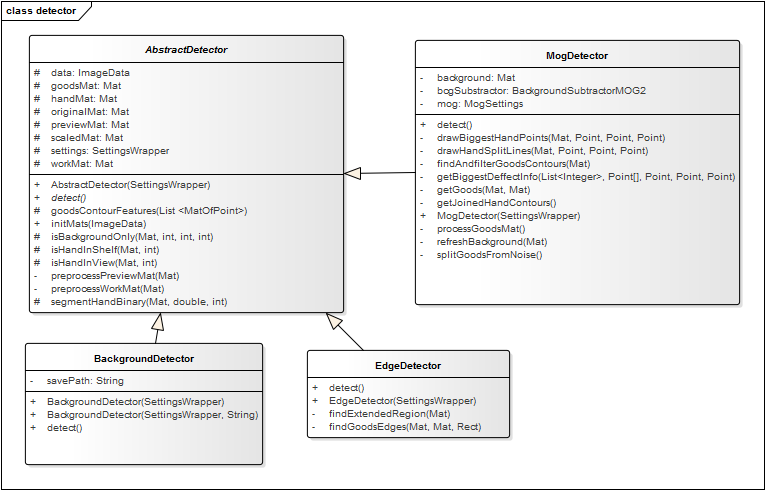
\includegraphics[width=1\textwidth]{images/ea_class_detector.png}
      \caption{Diagram tříd detekčních algoritmů}
      \label{fig:ea_class_detector}
    \end{figure} 
    
    \subsection{DataReciever}
    Pro příjem dat z~více zdrojů slouží abstraktní generická třída DataReciever. Jedním z~potomků této třídy je FlirDataReciever, který je využíván pro příjem dat z~termokamery a druhým potomkem je třída pro příjem z~webkamery nebo jiné USB kamery. Obě třídy implementují funkčnost ukládání a načtení snímků z~úložiště.

    \begin{figure}[h]
      \centering
      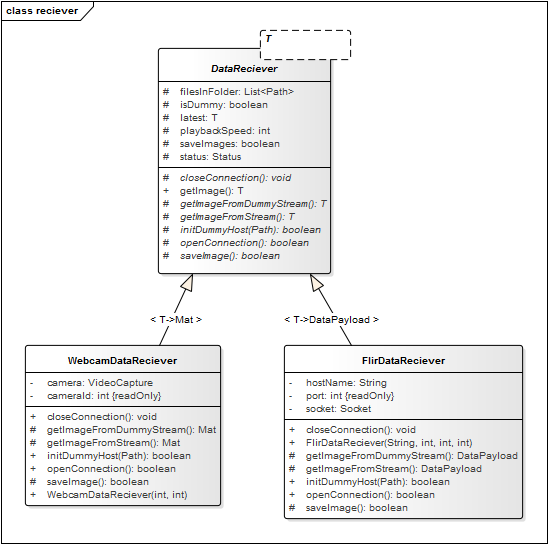
\includegraphics[width=1\textwidth]{images/ea_class_reciever.png}
      \caption{Diagram tříd zdrojů snímků}
      \label{fig:ea_class_reciever}
    \end{figure} 
    
    \subsection{Settings}
    V~paměti aplikace je uchováváno aktuální nastavení parametrů využívaných algoritmů. Tyto nastavení jsou rozděleny do čtyř skupin:
    \begin{description}
    \item [PreviewSettings] slouží k~aktivaci efektů algoritmů na náhledový snímek.
    \item [PreprocessingSettings] obsahuje jednotlivé parametry pro předzpracování obrazu před aplikací algoritmů.
    \item [MogSettings] jsou nastavení pro algoritmus odčítání pozadí.
    \item [EdgeDetectSettings] jsou nastavení parametrů algoritmu hranové detekce. Implementace těchto nastavení není dokončena.
    \end{description}
    Jednotlivé objekty nastavení jsou k~dispozici v~objektu SettingsWrapper, jehož instance je předávána všem detektorům. Všechna nastavení je možná exportovat do xml pomocí statické třídy SettingsManager.
    
    \begin{figure}[h]
      \centering
      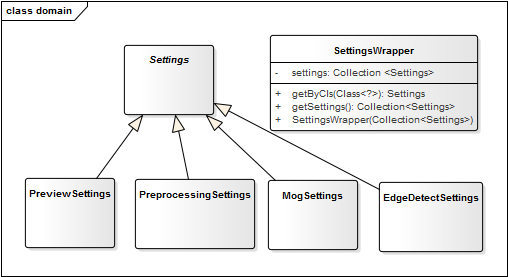
\includegraphics[width=1\textwidth]{images/ea_class_settings.png}
      \caption{Diagram tříd nastavení parametrů algoritmů}
      \label{fig:ea_settings}
    \end{figure} 

	\subsection{Práce s~obrazem}
    Poslední částí, která stojí za zmínku je balíček image, jehož obsahem jsou dvě statické třídy MatOperations a ImageConvertor. Třída MatOperations je pomocná třída pro práci s~OpenCV maticemi, která obsahuje volání knihovny, ale oproti běžnému volání nikdy nemodifikuje vstupní data. ImageConvertor obsahuje optimalizované metody pro převod mezi binárními daty, OpenCV maticemi a JavaFX obrázkem.

    \begin{figure}[h]
      \centering
      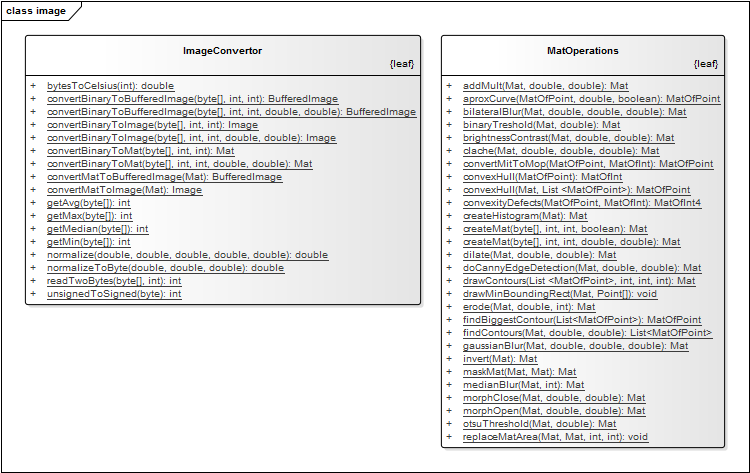
\includegraphics[width=1\textwidth]{images/ea_class_image.png}
      \caption{Diagram tříd baličku image}
      \label{fig:flir_binary_viewer}
    \end{figure} 


    \begin{figure}[h]
      \centering
      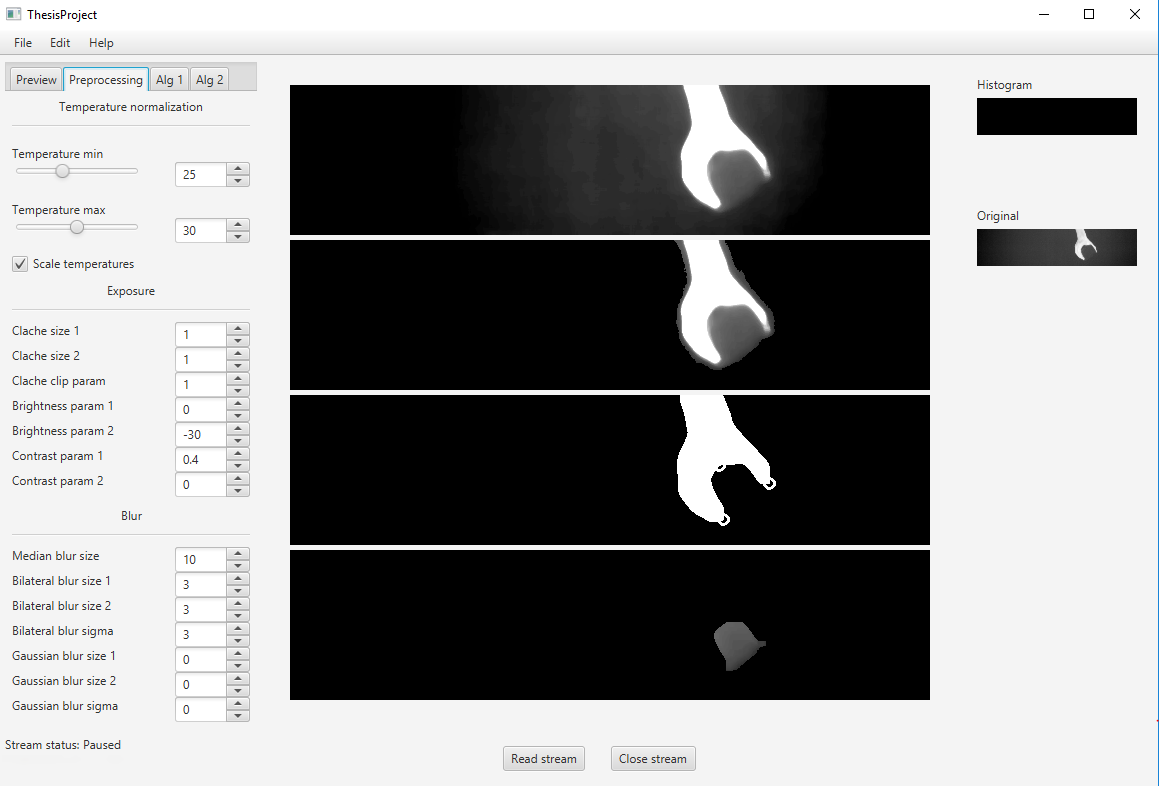
\includegraphics[width=1\textwidth]{images/main_app.png}
      \caption{Aplikace s~detekčními algoritmy}
      \label{fig:flir_binary_viewer}
    \end{figure} 
    
\clearpage

\section{Aplikace pro anotování snímků}
Pro potřeby vyhodnocování bylo nutné jednotlivé snímky rozdělit do skupin. K~tomu byl vytvořen tento nástroj, který lze snadno ovládat pomocí klávesnice a tím rychle rozřazovat jednotlivé snímky. 

Přesouvání mezi jednotlivými snímky probíhá pomocí klávesnicových šipek a přesunutí snímku do předem definované složky pomocí čísla 1-4 v~závislosti na kategorii. Snímky je též možné vyhledávat pomocí textového pole a pomocí klávesy D odstraňovat.

V~implementaci nejsou žádné složitosti. Aplikace se skládá pouze z~jednoho ovladače (MainController), který deleguje požadavky uživatelského rozhraní. Soubory jsou udržovány v~objektu InMemoryFiles, který snímky v~paměti spravuje a poskytuje je zpět do GUI podle nutnosti. Všechny metody pro převod binárního souboru na snímek poskytuje statická třída ImageConversions.

\begin{figure}[h]
  \centering
  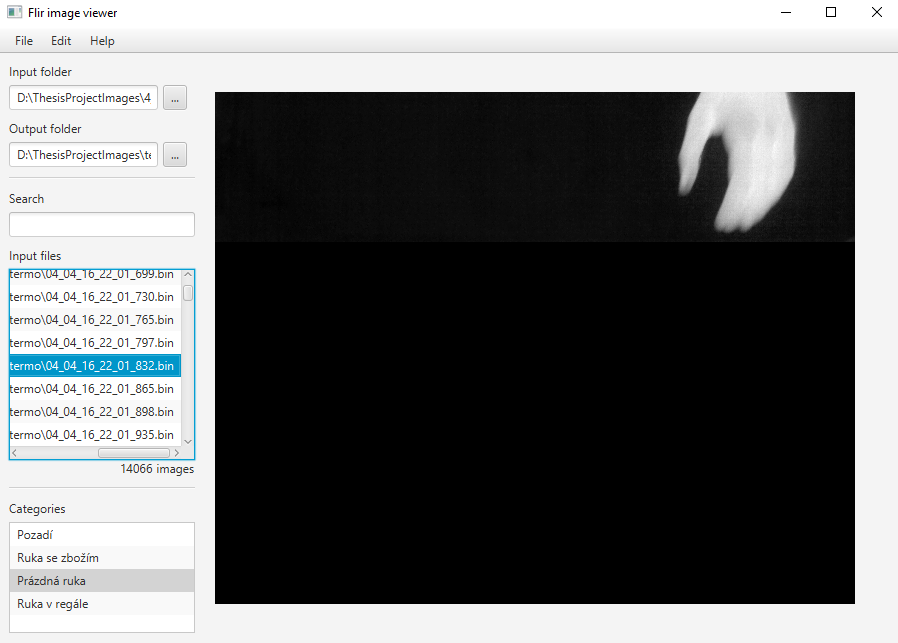
\includegraphics[width=1\textwidth]{images/flir_binary_viewer.png}
  \caption{Aplikace pro anotování snímků}
  \label{fig:flir_binary_viewer}
\end{figure} 